\documentclass[12pt]{article}
\usepackage{amsmath}
\usepackage{graphicx}
\usepackage{hyperref}
\usepackage[latin1]{inputenc}
\usepackage[top=2cm, bottom=2cm, left=2cm, right=2cm, headsep=14pt]{geometry}
\usepackage[T1]{fontenc}
\usepackage[utf8]{inputenc}
\usepackage{spverbatim}
\usepackage{float}
\title{Report 6 Gluster}
\author{Group 2}
% \author{Nguyen Vu Hung}
\begin{document}
\maketitle
  \section{Setup everything}
    \textbf{\large Install GlusterFS}\\
        Add the GlusterFS PPA 
        \begin{verbatim}
            sudo add-apt-repository ppa:gluster/glusterfs-3.13
        \end{verbatim}
        Update GlusterFS
        \begin{verbatim}
            sudo apt-get update
        \end{verbatim}
        Install GlusterFS
        \begin{verbatim}
           sudo apt-get install -y glusterfs-server
        \end{verbatim}
        
     \textbf{\large Create a trusted pool}\\
        Sometimes you have to configure the firewall before connecting. Use ifconfig to check your IP\\
        \begin{verbatim}
            sudo iptables -I INPUT -p all -s <ip-address> -j ACCEPT
        \end{verbatim}
            Note: When you input ip address, you do not need "< >" \\
            Add server to trusted pool
        \begin{verbatim}
           sudo gluster peer probe <ip-address>
        \end{verbatim}
        Check for all peer status to make sure you are connected
        \begin{verbatim}
           sudo gluster peer status
        \end{verbatim}   
        
    \textbf{\large Create a Distributed Replicated Volume}\\
        For server and each node make a storage to act as a brick. Do not grant the storage root permission\\
        For example
        \begin{verbatim}
            mkdir home/hung/gluster/test
        \end{verbatim}
        Create a distributed replicated volume
        \begin{spverbatim}
           sudo gluster volume create <volume name> replica <int> transport tcp <ip server1>:<path of brick server 1> <ip server2>:<path of brick server 2> ... force
        \end{spverbatim}
        \\Number of bricks is not a multiple of replica count <int>. For example\\
         \textbf{\small sudo gluster volume create test replica 2 transport tcp 
         192.168.0.160:/home/hung/gluster/test 192.168.0.175:/home/lezardvaleth97/gluster/test force}
        \\Start the volume
        \begin{verbatim}
            sudo gluster volume start <volume name>
            sudo gluster volume start test
        \end{verbatim}
        \textbf{Setup clients}\\
        Each client have to install GlusterFS client
        \begin{verbatim}
            sudo apt-get install -y glusterfs-client
        \end{verbatim}
        Create a directory to mount glusterfs flies to client (use mkdir) then mount
        \begin{verbatim}
            sudo mount -t glusterfs <ip address>:/<volume name> <directory>
            sudo mount -t glusterfs 192.168.0.160:/test /glusterfs
        \end{verbatim}
        u can check if the system if mounted or not by
        \begin{verbatim}
            df -h
        \end{verbatim}
        From now, you should be able to transfer file from each node. Copy the file to the volume then it's done\\
        To check the volume status
        \begin{verbatim}
            sudo gluster volume info
        \end{verbatim}
 
    \section{Perform benchmark}
    To perform benchmark, we use iozone. Firstly, install iozone
        \begin{verbatim}
            sudo apt install iozone3
        \end{verbatim}
        Then
        \begin{verbatim}
            sudo iozone -r 1k -i 0 -i 1 -i 2 -t 4 -s 128M
        \end{verbatim}
        Where -r 1k is to set record size 1kB
        -i 0 is used to test random write/rewrite, -i 1 is used  to test read/reread and -i 2 is used test write/read.\\
        -t 8 is used to set number of threads to 8 (since I'm using laptop with 8 threads)\\
        -s 128MB is to used set specify the size of test at 128MB.\\
        \\
        Theses are the results
    \begin{figure}[H]
        \centering
       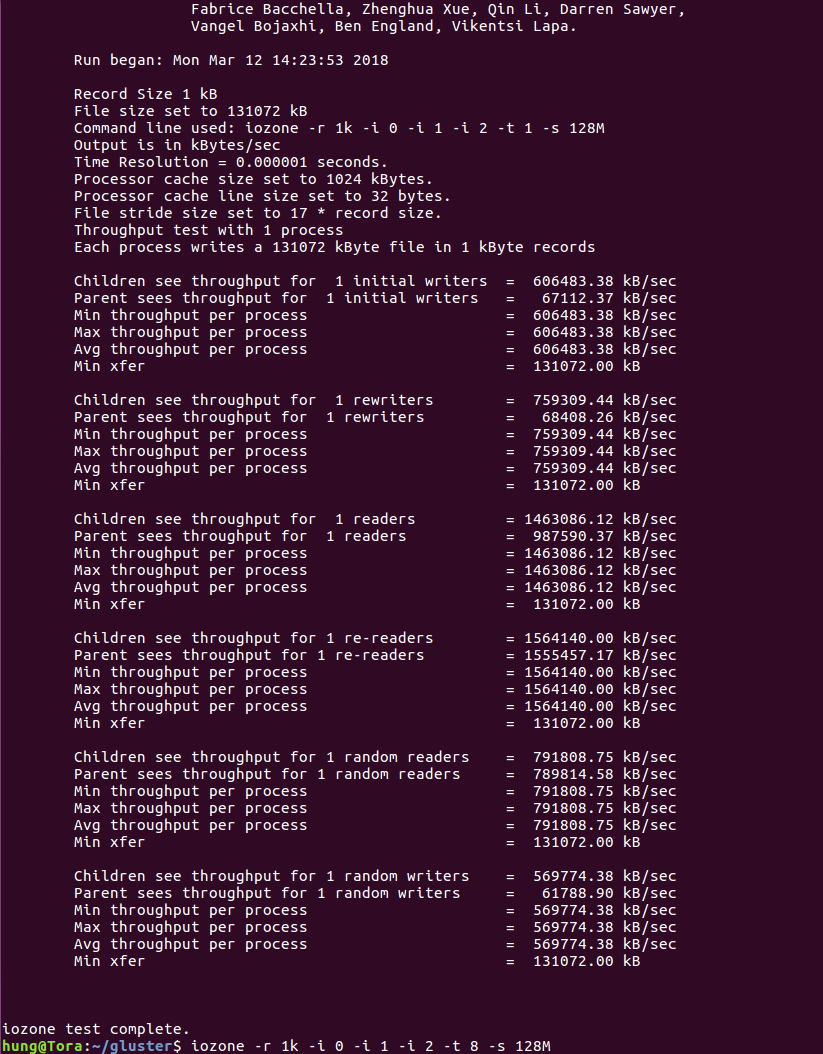
\includegraphics[scale=0.4]{1kB 1 proccesses.png}
       \caption{record size 1kB with 1 threads}
    \end{figure}
     \begin{figure}[H]
        \centering
       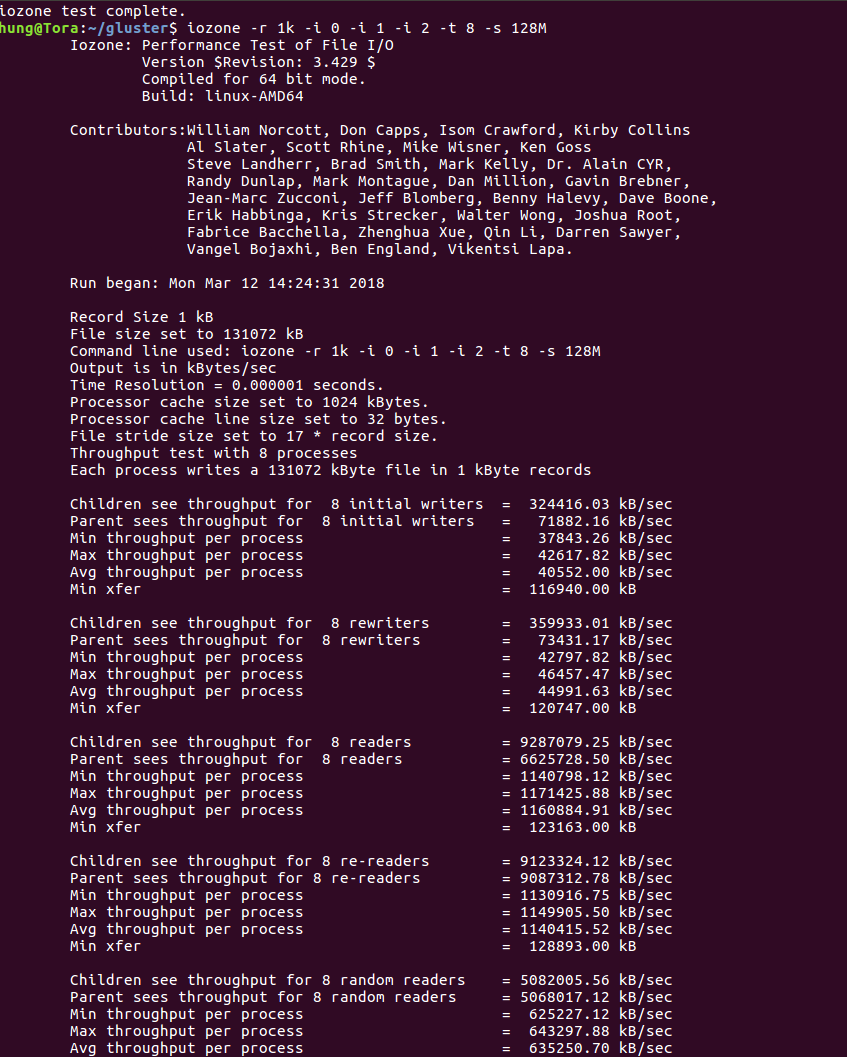
\includegraphics[scale=0.4]{1kB 8 proccesses.png}
       \caption{record size 1kB with 8 threads}
    \end{figure}
     \begin{figure}[H]
        \centering
       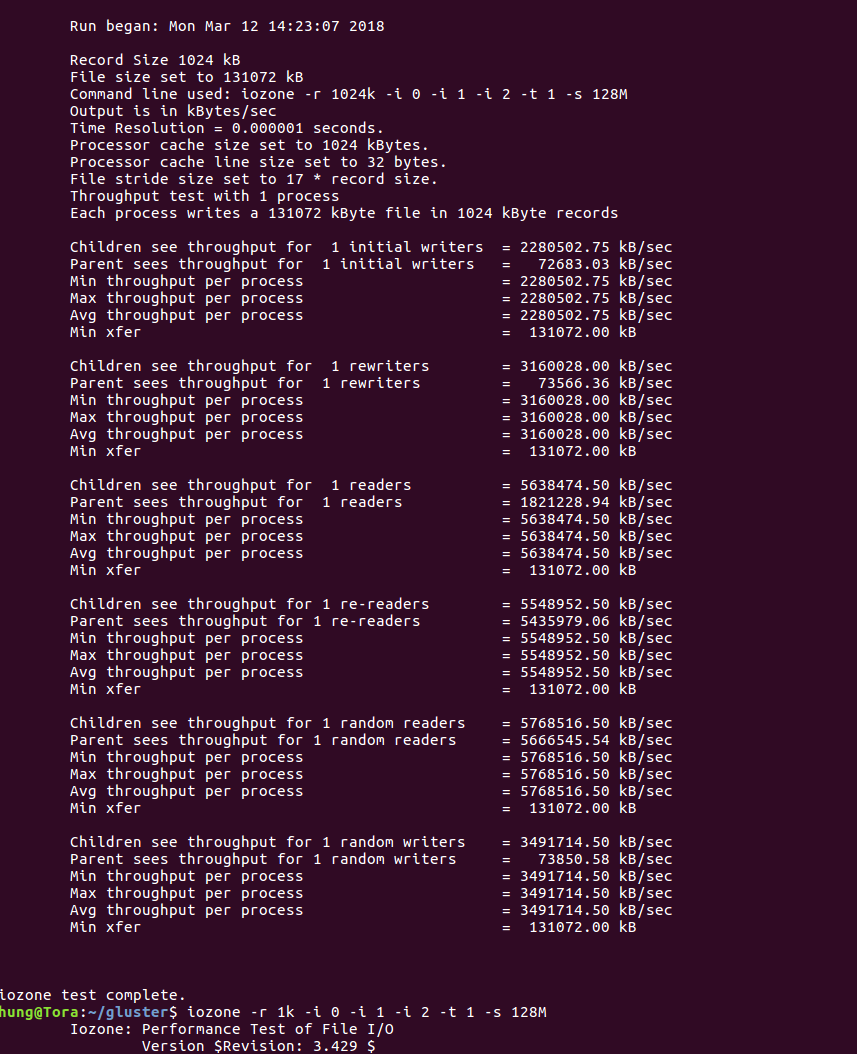
\includegraphics[scale=0.4]{1024kB 1 proccesses.png}
       \caption{record size 1028kB with 1 threads}
    \end{figure}
     \begin{figure}[H]
        \centering
       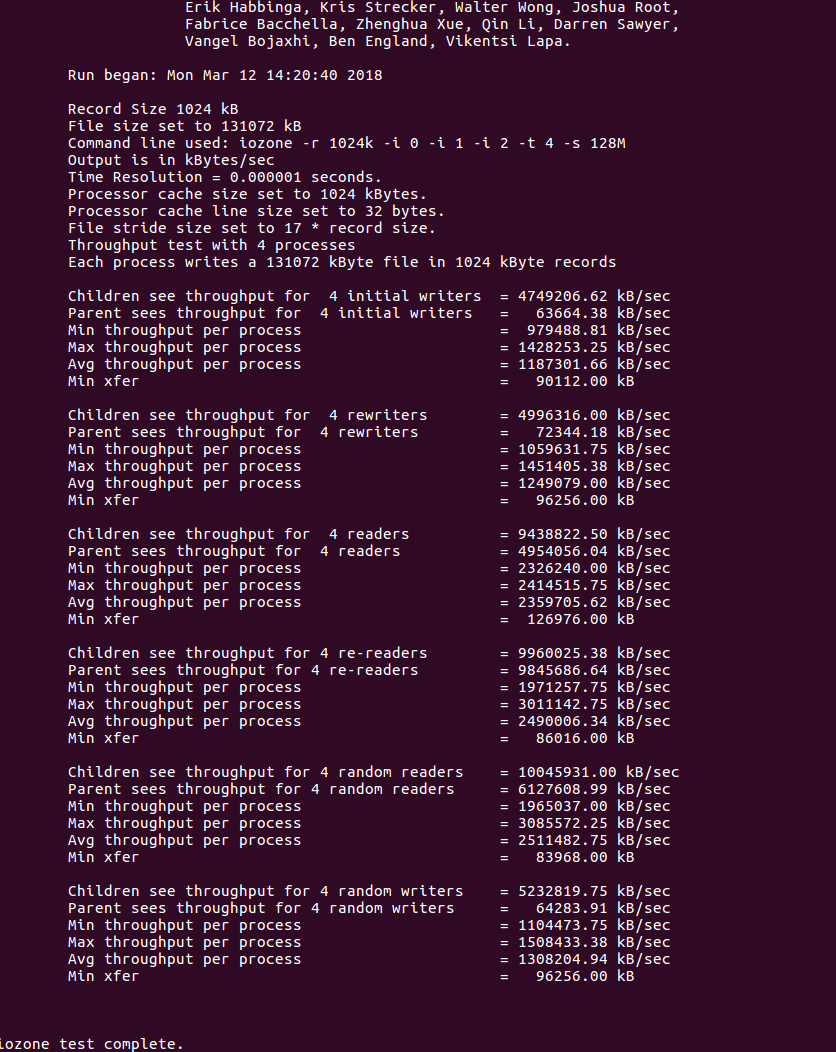
\includegraphics[scale=0.4]{1024kB 4 proccesses.png}
       \caption{record size 1024kB with 4 threads}
    \end{figure}
     \begin{figure}[H]
        \centering
       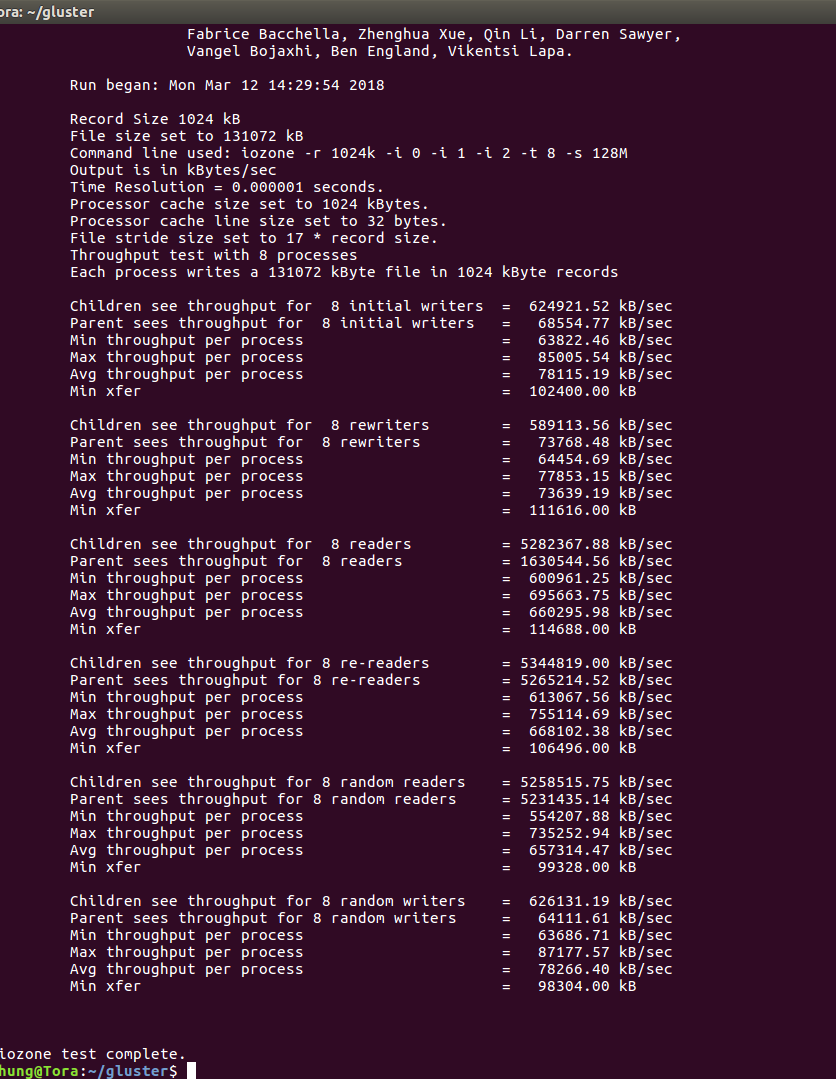
\includegraphics[scale=0.4]{1024kB 8 proccesses.png}
       \caption{record size 1024kB with 8 threads}
    \end{figure}
        We can see that glusterfs reads and writes faster with files with large size.\\
        The more threads, the slower it reads/writes. The reading speed of glusterfs is also faster than writing speed.
        \\ Note: We used local area network to test.
        
    \section{Who does what}
Nguyen Vu Hung did and wrote the report
\end{document}
